\chapter{Formal Security Analysis of Three Key Establishment Protocols}
\label{chp:analysis}


\section{Modelling Security Properties}

As mentioned in Section \ref{sec:attributes}, key establishment schemes desire certain security properties. In the verification of the security protocols of this thesis, the following properties are verified: \emph{Entity authentication}, \emph{Implicit key authentication}, \emph{Explicit key authentication}, \emph{Known-key secrecy}, \emph{Key control}, and \emph{Secrecy of key}. As mentioned in Section \ref{sec:attributes}, symmetric key establishment schemes are not resilient against \gls{kci} attacks, and do not provide forward secrecy. These properties are nevertheless included in the models as \gls{sakes} uses a lightweight version of public-key cryptography and the type of Diffie-Hellman key agreement to establish session keys.

\paragraph{Entity authentication} Entity authentication between nodes corresponds to the security claim \texttt{Alive}, and can also be verified through stronger claims such as \texttt{Weakagree}. This property can only be violated if the adversary is able to inject or tamper with messages that are transmitted over the network, which we assume that the adversary in a \gls{6lowpan} network is.

\paragraph{Implicit key authentication} Implicit key authentication is modelled through the settings of the adversary compromise model described in Section \ref{sec:adversary}. The property is modelled by allowing the adversary to obtain the long-term keys and impersonate anyone except for the nodes that are supposedly establishing keys.

\paragraph{Explicit key authentication} Is achieved when the protocol satisfied both implicit key authentication and key confirmation. This is modelled through the security claim for non-injective agreement denoted as \texttt{ni-agree}, but can also be modelled by using \texttt{running} and \texttt{commit} claims.

\paragraph{Known-key security} By revealing session keys to the adversary after usage (i.e. the session key is expired, and will never be used again) known-key security can be modelled. This is done by setting the \emph{Session-key reveal} rule in the adversary compromise model.

\paragraph{Key control} Scyther has no support for verifying key control. Therefore, this security property has to be verified by hand. 

\paragraph{Secrecy of key} To model a key (or any other property) as secret, the \texttt{secrecy} claim is used in Scyther.

\paragraph{Forward secrecy} Both \gls{pfs} and \gls{wpfs} are related to active adversaries, and is modelled through the adversary compromise model, which can be configured to leak the long-term private key which the session keys are derived from.

\paragraph{Key compromise impersonation} \gls{kci} is also a property related to an active adversary, and is therefore available through the adversary model where the adversary can be allowed to obtain the long-term private key of the actors.


\section{Formal Security Analysis of APKES}
\label{sec:apkes-analysis}

\gls{apkes} is modelled as two roles, the initiator $A$ and the responder $B$, agreeing upon a pairwise key through the message exchange that is presented in Figure \ref{fig:apkes-handshake}. There is not specified any concrete type of pluggable scheme (i.e. the scheme where \gls{apkes} obtains the shared secret between two nodes), hence we assume that whatever scheme is used is secure. In the model, the shared secret obtained from the pluggable scheme has been modelled using Scyther's built-in support for shared symmetric keys, where the two nodes $A$ and $B$ both possesses the shared secret at start-up.

\gls{apkes} states that the $R_A$ value has to be checked whether or not it has been tampered with, before the pairwise key can be derived at the initiating side. This can be verified by modelling the protocol to agree upon the $R_A$ value during the protocol execution, and committing to this. In addition, we model agreement over the pairwise key by using a \texttt{Running} claim in role $B$ after receiving the \texttt{ACK} authenticated with the pairwise key, and \texttt{Commit} claims in both roles to claim explicit key authentication on the pairwise key. As $B$ authenticates the $HELLOACK$ by using the shared secret, we do not claim that the pairwise key is created before $A$ receives the $HELLOACK$ from B. The Scyther model of \gls{apkes} can be viewed in its entirety in Appendix \ref{app:apkes}.

\subsection{Security Claims}

By taking starting point in the protocol specification from Section \ref{subsec:apkes-spec} and the alleged security properties from Section \ref{subsec:apkes-prop}, the protocol is modelled as an \gls{spdl}-script, which can be verified by Scyther. Listing \ref{lst:claims-a-apkes} describes the various security claims that is chosen for $A$. In these claims, we verify that the other party in the protocol is authentic, and that the pairwise key is secret. Claims for non-injective synchronization and agreement is also added to verify that the protocol executes as expected. The security claims for role $B$ in \gls{apkes} are stated in Listing \ref{lst:claims-b-apkes}. Compared to the claims for $A$, $B$ does not contain the \texttt{Commit} claim for the variable $N_A$, as the \texttt{Running}, \texttt{Commit} approach is used in role $A$ to provide agreement (i.e. confirm that the nonce has not been altered by $B$) over the nonce $N_A$. We also claim non-injective synchronization and agreement.\\

\begin{lstlisting}[caption={Security claims for role A in APKES.}, label={lst:claims-a-apkes}]
	claim(A, Alive);
	claim(A, Weakagree);
	claim(A, Niagree);
	claim(A, Nisynch);
	claim(A, Commit, B, Na);
	claim(A, Secret, PairwiseKey);
	claim(A, Commit, B, PairwiseKey);
\end{lstlisting}


\begin{lstlisting}[caption={Security claims for role B in APKES.}, label={lst:claims-b-apkes}]
	claim(B, Alive);
	claim(B, Weakagree);
	claim(B, Niagree);
	claim(B, Nisynch);
	claim(B, Secret, PairwiseKey);
	claim(B, Commit, A, PairwiseKey);
\end{lstlisting}


\subsection{Adversary}

In the description of \gls{apkes}, no specific adversary is mentioned. We assume that such a protocol would be used for key establishment in \gls{6lowpan} networks, which are potentially deployed in hostile areas. Therefore, we can assume that the adversary would be able to observe, inject, and tamper with messages that are sent over the network. As \gls{apkes} does not utilize any session keys, but rather agreeing upon a fixed long-term key, we model the adversary in a Dolev-Yao way without giving it any active capabilities other than being able to obtain the long-term keys of nodes not participating in the current key establishment process. 

\subsection{Results}

Figure \ref{fig:apkes-verified} shows the verification result from running the model of \gls{apkes} through Scyther in the presence of the adversary described above. Scyther was able to perform an unbounded verification of the model where all claims but one were successfully verified. \gls{apkes} provides verifiable entity authentication, explicit key authentication for role $B$ (implicit for $A$), and holds the non-injective synchronization property, which means that every message in protocol is executed as expected, even in the presence of the adversary. When looking at the characterization of the protocol, there exist only one executable trace for each of the roles. Hence, there does not exist any malicious behaviour that can force the modelled protocol to misbehave. The attack proposed by Scyther on $Commit\ B, \{Na, Nb\}k(A,B)$ is not a direct attack on the protocol, but it shows that it is not possible to achieve explicit key authentication for the role $A$, as it has no knowledge of if $B$ has computed the pairwise key. 


\begin{figure}[h]
	\centering
	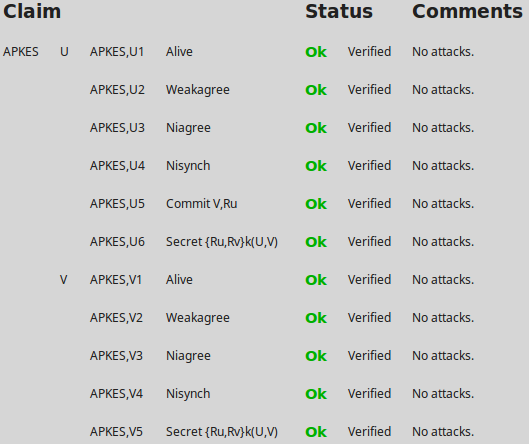
\includegraphics[scale=0.75]{analysis/apkes-verified.png}
	\caption{Result of verifying APKES' security claims using Scyther.}
	\label{fig:apkes-verified}
\end{figure}



\section{Formal Security Analysis of AKES}
\label{sec:akes-analysis}

\gls{akes} is modelled almost as its predecessor, but with additional content that is used to allow mobility for the devices. As \gls{akes} is used for establishing session keys, the \texttt{SKR} claim is used emphasize that the key is in fact a session key. The pluggable scheme is assumed to be secure, and is modelled as a symmetric key shared between the two communicating parties using Scyther's built-in symmetric key support. Appendix \ref{app:akes} contains the model in its entirety. \gls{apkes} was not able to provide explicit key authentication of role $B$ for the initiator $A$. In \gls{akes}, however, the received \texttt{HELLOACK} is authenticated using the session key. Therefore, we model a \texttt{Running} claim (not present in Listing \ref{lst:claims-a-akes} or \ref{lst:claims-b-akes} - See Appendix \ref{app:akes}) to indicate that the role $B$ has computed the key at this point in time and a \texttt{Commit} claim to state that the two parties agree that the session key has been computed.

\subsection{Security Claims}

From the protocol specification in Section \ref{subsec:akes-specs} and the assumed security properties in Section \ref{subsec:akes-props}, the security claims that are claimed to hold for the two roles in \gls{akes} are listed in Listing \ref{lst:claims-a-akes} and Listing \ref{lst:claims-b-akes}. In addition to claiming authentication for the other party, we also claim that the protocol has been executed as intended by adding claims for non-injective synchronization and agreement.\\

\begin{lstlisting}[caption={Security claims for role A in AKES.}, label={lst:claims-a-akes}]
	claim(A, SKR, SessionKey);
	claim(A, Alive);
	claim(A, Weakagree);
	claim(A, Niagree);
	claim(A, Nisynch);
	claim(A, Commit, B, SessionKey);
\end{lstlisting}


\begin{lstlisting}[caption={Security claims for role B in AKES.}, label={lst:claims-b-akes}]
	claim(B, SKR, SessionKey);
	claim(B, Alive);
	claim(B, Weakagree);
	claim(B, Niagree);
	claim(B, Nisynch);
	claim(B, Commit, A, SessionKey);
\end{lstlisting}

\subsection{Adversary}

The adversary in this model is nearly the same adversary as the one introduced in the verification of \gls{apkes}. However, in order to model session keys, the adversary is allowed to obtain all session keys whose identifier differs from the current protocol execution. 

\subsection{Results}

Figure \ref{fig:akes-verified} shows the result of running the model of \gls{akes} through Scyther in the presence of the adversary presented above, where \gls{akes} is verified for an unbounded state space and all the claimed security properties are successfully verified. \gls{akes} provides provable authentication for both roles, as well as explicit key authentication. In addition, \gls{akes} is proved to hold the non-injective synchronization and data agreement claims which state that the protocol was executed as intended. When looking at the characterization of \gls{akes} only one possible trace is returned for each role, which means that there exists only one way to execute the protocol.

\begin{figure}[h]
	\centering
	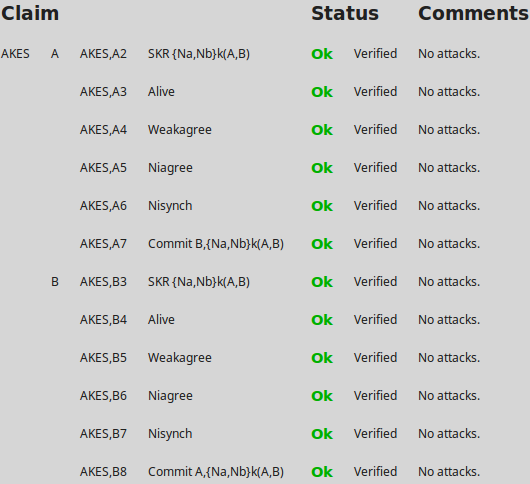
\includegraphics[scale=0.95]{analysis/akes-verified.png}
	\caption{Result of verifying AKES' security claims using Scyther.}
	\label{fig:akes-verified}
\end{figure}


\section{Formal Security Analysis of SAKES}
\label{sec:sakes-analysis}

From the protocol specification in Section \ref{subsec:sakes-spec} and the assumed security properties in Section \ref{subsec:sakes-props}, \gls{sakes} have been modelled into four roles: $A$ (End device), $B$ (Router), $C$ (Border router), and $D$ (Server). The authentication phase is carried out between $A$, $B$, and $C$, before $B$ and $D$ establish the session key, which is distributed from the router $B$ to the end device $A$. As the protocol specification presented in the original protocol proposal can be considered inconsistent, some assumptions have been made in the model.

The verification of the original protocol in its entirety takes over 72 hours to complete on a workstation with an Intel Core i7 processor with four cores and 12 GB \gls{ram} (The experiment was aborted at this point). Therefore, it has been infeasible to formally verify the complete protocol in one round, hence the two phases have been separated into different models to be able to provide some insight on the weaknesses of \gls{sakes}. The two models are available in Appendix \ref{app:sakes-auth} and \ref{app:sakes-keys}. There may, however, be additional attacks on the protocol that the analysis of these models is unable to detect. Especially as the nonces $N_A$, $N_B$, and $N_C$ are re-used in the key establishment phase, but the models are unable to link these values between protocols, the usage of these nonces in the key establishment phase may lead to attacks as they are freshly generated.


\subsection{Authentication Phase}
\label{subsec:sakes-auth}

\subsubsection{Security Claims}

The end device $A$ is only in direct communication with the router $B$ and the border router $C$, which is why authentication is only claimed for these two roles as seen in Listing \ref{lst:claims-a-sakes-auth}. We add claims for non-injective synchronization and agreement to find attacks where the messages are not exchanged as intended.\\

\begin{lstlisting}[caption={Security claims for role A during the authentication phase in SAKES.}, label={lst:claims-a-sakes-auth}]
	claim(A, Alive, B);
	claim(A, Alive, C);
	claim(A, Weakagree, B);
	claim(A, Weakagree, C);
	claim(A, Niagree);
	claim(A, Nisynch);
\end{lstlisting}


Listing \ref{lst:claims-b-sakes-auth} contains the claims that are stated for role $B$ (i.e. the \gls{6lowpan} router) in \gls{sakes} during the authentication phase. The router is originally interacting with all the other entities in the network, but during the authentication it only interacts with the end device $A$, and the border router $C$. Hence we are claiming authentication for only these roles. In addition, we state that the ephemeral key $Sk_B$, which is generated by the border router during the authentication phase and which is to be used in the key establishment, is secret. To verify that the role behaves as intended, we add claims for non-injective synchronization and agreement.\\

\begin{lstlisting}[caption={Security claims for role B during the authentication phase in SAKES.}, label={lst:claims-b-sakes-auth}]
	claim(B, Secret, Sk);
	claim(B, Alive, A);
	claim(B, Alive, C);
	claim(B, Weakagree, A);
	claim(B, Weakagree, C);
	claim(B, Niagree);
	claim(B, Nisynch);
\end{lstlisting}

The border router $C$ does only participate in the authentication phase with $A$ and $B$, hence we claim authentication for these two parties. In addition we add claims for non-injective synchronization and agreement to state that the protocol was executed as expected as seen in Listing \ref{lst:claims-c-sakes-auth}.\\

\begin{lstlisting}[caption={Security claims for role C during key establishment in SAKES.}, label={lst:claims-c-sakes-auth}]
	claim(C, Alive, A);
	claim(C, Alive, B);
	claim(C, Weakagree, A);
	claim(C, Weakagree, B);
	claim(C, Niagree);
	claim(C, Nisynch);
\end{lstlisting}

\subsubsection{Adversary}

For the authentication phase in \gls{sakes} we assume a Dolev-Yao adversary which is capable of eavesdropping, delete messages, compute cryptographic analysis on intercepted messages, forge new messages from its knowledge, and insert them into the network. 

\subsubsection{Results}

Figure \ref{fig:sakes-verified-auth} shows the result of verifying \gls{sakes}' authentication phase, where multiple of the claimed security properties are falsified. Scyther is able to verify that \gls{sakes} provides entity authentication for the end device, router, and border router, but fails to provide stronger notions of authentication such as weak agreement for the end device. Also, the authentication phase in \gls{sakes} does not provide non-injective synchronization nor non-injective data agreement for either of the three roles. The attacks presented below are described more thoroughly in Section \ref{subsec:sakes-fix}, and improvements are suggested to achieve the claimed security properties.

\begin{list}{•}{}

\item \texttt{SAKES\_AUTH, A3 \& A4 Weakagree B \& C}: The attacks proposed by Scyther that falsifies the \texttt{weakagree} claims for the end device leverage the last message that is sent between the end device and the border router, and can be seen in Appendix \ref{fig:sakes-attack-weakagree}. When the border router receives the relayed request from router, it has to confirm the identity of the router to the end device. There are, however, flaws in the messages that are exchanged, which enables an adversary to use the request created by the end device and the nonce generated by the router to change a different end device's perception of its closest router.

\item \texttt{SAKES\_AUTH, A6 \& B7 \& C6 Nisynch}: Neither $A$, $B$, or $C$ is able to hold the non-injective synchronization property. If we study the attack proposed in Appendix \ref{fig:sakes-attack-nisynch}, we see that the adversary is using the same approach as in the attack on the \texttt{weakagree} above. In the original protocol description of \gls{sakes}, the adversary is able to combine the information sent in the second and third message into a message that is sent directly to the border router. Such an alternation is the message flow is not allowed in the model of the protocol, and hence the \texttt{nisynch} properties are falsified.

\item \texttt{SAKES\_AUTH, A6 \& B7 \& C6 Niagree}: Scyther also proposes attacks targeting the non-injective agreement claims. These attacks are of the same flavour as the attacks targeted at the \texttt{nisynch} property above, and the claims are falsified as the adversary is able to combine information in observed messages into valid new messages. Generation of new messages lead to a different set of data items, hence the protocol is not able to agree upon the data that is exchanged throughout the protocol.

\end{list}

\begin{figure}[h]
	\centering
	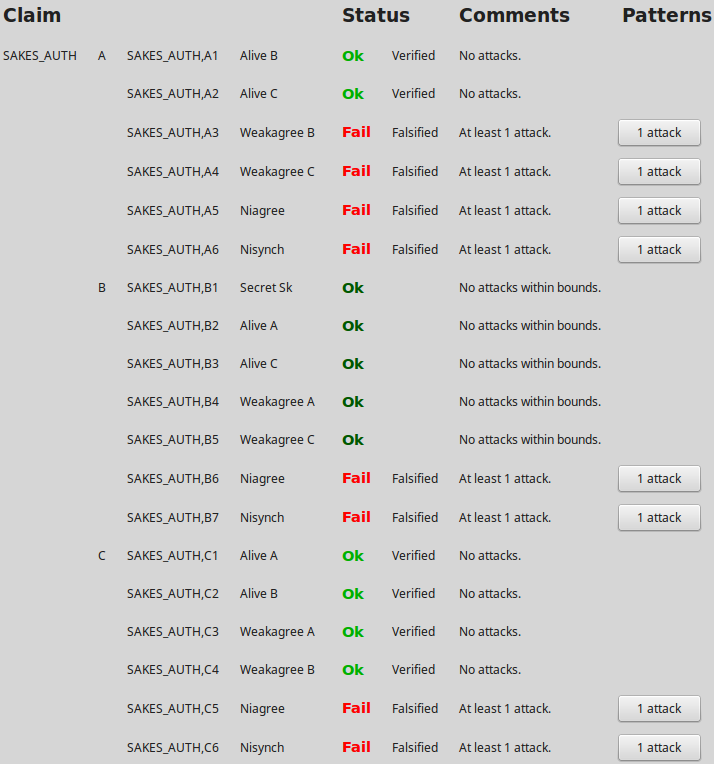
\includegraphics[scale=0.68]{analysis/sakes-auth-verified.png}
	\caption{Result of verifying SAKES' authentication claims using Scyther.}
	\label{fig:sakes-verified-auth}
\end{figure}

\newpage

\subsection{Key Establishment Phase}

In order to model the key establishment phase in \gls{sakes}, it is assumed that the Diffie-Hellman key agreement is done correctly by letting $B$ and $D$ share their secret key to the power of the generator $g$. In addition, it is assumed that when the authors use notion of ``decrypting the ciphertext encrypted with the private key of $X$'', they actually mean that the message is signed using the private key of $X$, and that the signature can be verified by applying the corresponding public key. When it comes to the notation of \gls{mac-auth}s, an assumption is that the alleged \gls{mac-auth} that is sent between the router and the server that do not share any symmetric key is simply a hash of the message.

Originally, the server distributes the generator $g$ and the prime modulus $P$ to the router. This means that a new message needs to be introduces to allow for the Diffie-Hellman procedure to be executed correctly. If the router $B$ either has the these two cryptographic numbers preloaded in its memory, or if they get distributed from the border server, the router is able to send $g^{Sk_B}$ to the server in its first message. As the original protocol specification got the Diffie-Hellman part wrong, the models presented in this section assume that the router has access to both $g$ and $P$ before initiating the key establishment process with the remote server $D$.


\subsubsection{Security Claims}

The session key establishment in \gls{sakes} is conducted between the router $B$ and the server $D$, before the session key is distributed from the router to the end device $A$. We assume that $A$ and $B$ have authenticated each other before the key establishment process is engaged. Listing \ref{lst:claims-a-sakes-key} shows the claims that is stated for the end device in the key establishment phase of \gls{sakes}. Since the only message that is sent between the two contains the session key, which is encrypted with their shared symmetric key $K_{A,B}$, we assume that the session key is secret by using the \gls{skr} claim. In addition, claims for non-injective synchronization and agreement have been added to ensure that the protocol is executing as expected based on the model.\\

\begin{lstlisting}[caption={Security claims for role A during key establishment in SAKES.}, label={lst:claims-a-sakes-key}]
	claim(A, Niagree);
	claim(A, Nisynch);
	claim(A, SKR, SessionKeyA);
\end{lstlisting}

As the router generates the session key on behalf of the end device $B$, we also state that the session key should be secret at the router side using the \gls{skr} claim as seen in Listing \ref{lst:claims-b-sakes-key}. As the router interacts with the remote server $D$, we also add claims for entity authentication. Finally, claims for non-injective synchronization and data agreement are added to verify that the protocols behaves as specified in the protocol model. \\

\begin{lstlisting}[caption={Security claims for role B during key establishment in SAKES.}, label={lst:claims-b-sakes-key}]
	claim(B, Alive, D);
	claim(B, Weakagree, D);
	claim(B, Niagree);
	claim(B, Nisynch);
	claim(B, SKR, SessionKeyA);
\end{lstlisting}


For the remote server, authentication is claimed only between it and the router which is establishes session keys with. The end device is indirectly authenticated through the proof that is signed by the authentication module in the border router, but this is not modelled as a direct authentication claim in this model. The generated session key $SessionKeyD$ is claimed to be secret using the \texttt{SKR} notation. In addition, we also claim non-injective synchronization and agreement for the role as seen in Listing \ref{lst:claims-d-sakes-key}.\\


% run verification with Alive, Weakagree, for A?
\begin{lstlisting}[caption={Security claims for role D during key establishment in SAKES.}, label={lst:claims-d-sakes-key}]
	claim(D, Alive, B);
	claim(D, Weakagree, B);
	claim(D, Niagree);
	claim(D, Nisynch);
	claim(D, SKR, SessionKeyD);
\end{lstlisting}

\subsubsection{Adversary}

For the key establishment phase, we assume a Dolev-Yao adversary which is capable of eavesdropping, delete messages, compute cryptographic analysis on intercepted messages, forge new messages from its knowledge, and insert them into the network. It is allowed for the adversary to obtain the session keys for all sessions whose identifier differs from the current session's identity. As \gls{sakes} utilizes a form of Diffie-Hellman key agreement, it is also assumed that the protocol should possess forward secrecy, especially since the half of the key is fixed as the remote server uses a permanent public key pair.

\subsection{Results}

The results of verifying the model of the key establishment phase in \gls{sakes} using Scyther is presented in Figure \ref{fig:sakes-verified-keys}. Entity authentication of both the router and the server is provided and verified in the key establishment process, but stronger notion such as \texttt{Weakagree} for the server $D$ is falsified for the router $B$ in this model. Both non-injective synchronization and data agreement are falsified for each of the roles in the key establishment phase. \gls{sakes} achieves known-key secrecy of the computed session key for both the router and the server, as well as the end device who receives the session key from the router.  If the model is run in presence of an adversary that is allowed to obtain the long-term private key, the generated session key is falsified, as \gls{sakes} does not provide forward secrecy.

\begin{figure}[h]
	\centering
	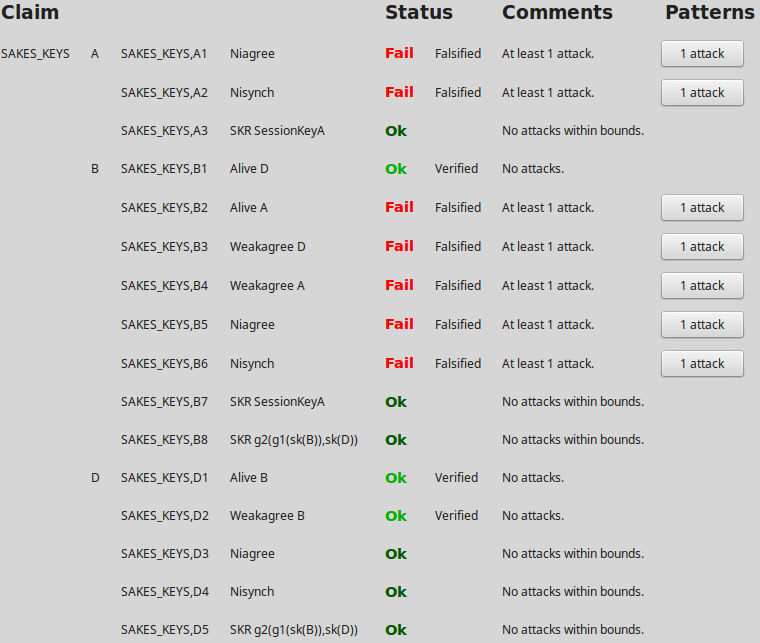
\includegraphics[scale=0.65]{analysis/sakes-keys-verified.png}
	\caption{Result of verifying SAKES' key establishment claims using Scyther.}
	\label{fig:sakes-verified-keys}
\end{figure}

\begin{list}{•}{}

\item \texttt{SAKES\_KEYS, A2 \& B4 \& D4 Nisynch}: The attacks on the non-injective synchronization claim are shown in Figure \#. In this attack, the adversary extracts the proof from the intercepted message, and generates its own public key pair and nonces in order to 	forge a message to the remote server. However, as the server verifies the identities within the the proof it is questionable whether this attack manifests in a full-size model of the protocol which includes both phases.

\item \texttt{SAKES\_KEYS, A1 \& B3 \& D3 Niagree}:

\item \texttt{SAKES\_KEYS, B2 Weakagree D}: Because the proof is not returned.
\end{list}


\section{Limitations in the Analysis}

Even though Scyther is a powerful tool for formal security analysis, there are certain types of attacks that it is not able to model. Replay attacks, where the adversary saves a captured frame for injecting it into the network at a later time, are not possible to model in Scyther. Both \gls{akes} and \gls{apkes} claim to avoid replay attacks through the 802.15.4 security sub-layer and the use of frame counters to discover frames that have been previously observed \cite{krentz2015handling, krentz20136lowpan}.

\gls{sakes} claims to prevent replay attacks by adding nonces and \gls{mac-auth}s to prevent messages from being tampered with and to ensure freshness \cite{hussen2013sakes}. This analysis does not, however, verify these claims. As the \gls{sakes} protocol proved to be computational expensive to verify on the available equipment, it has been divided into two separate protocols. While the analysis finds certain attacks on the two phases, there may be additional attacks that the models are unable to detect.

The big weakness with this analysis is that the mutual authentication that is achieved between $A$, $B$, and $C$ in the authentication phase is not transferable to the key establishment phase. Therefore, the necessary values are freshly generated at the appropriate places. For example are the nonce $N_C$ generated at the router $B$ before the router sends its first message in the key establishment phase.  


% Litt mer?

%For example could an adversary be able to establish the session key with a different entity than what was originally intended.



% How to check for properties:

% Forward Secrecy: Not able to achieve in symmetric key. Check through Scyther rules.

% Known-Key Security: Session-Key reveal

% Key Confirmation: running, commit / niagree

% Key Compromise Impersonation: Impossible to achieve in protocols relying on symmetric keys? Need asymmetric? Boyd book. SKR claim of an entity whose long-term key is revealed to the adversary

% Unknown key share: Known-Key Security?

% Entity authentication: From A to B: Aliveness of A in B's claims.

% Implicit: Long-term reveal for other entities than A and B.

% Explicit. Implicit + key confirmation




%As \gls{sakes} uses Diffie-Hellman, which Scyther does not originally support, a ``hack'' has been introduced to enable Scyther to interpret $(g^a)^b$ and $(g^b)^a$ as equal. Diffie-Hellman can be modelled by introducing a helper protocol in Scyther that underapproximates $g^{x}$ into $hashfunction(g, x)$. The helper protocol is shown in Listing \ref{lst:helper} and is marked with the at-symbol (@). This allows Scyther to interpret the two terms $g2(g1(T1),T2)$ and $g2(g1(T2), T1)$ as approximate equal \cite{scyther-manual}.\\
%
%\begin{lstlisting}[caption={Helper protocol to model Diffie-Hellman in SAKES.}, label={lst:helper}]
%hashfunction g1, g2;
%
%protocol @exponentiation(DH)
%{
%	role DH
%	{
%		var T1,T2: Ticket;
%
%		recv_!1(DH, DH, g2(g1(T1),T2) );
%		send_!2(DH, DH, g2(g1(T2),T1) );
%	}
%}
%\end{lstlisting}
